\chapter{Result}

The first analysis that we will do is a comparison between the liner method and the Bertalmio et al.

To do this comparison we use the image \eqref{Pori}.

\begin{figure}[h]
\centering
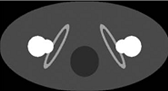
\includegraphics[scale=1.2]{img/Pori}
\caption{{Real Hip Phantom}}\label{Pori}
\end{figure}

The image \eqref{Pori} represent a hip phantom with bilateral prostheses. However, this is the real image, when we do the tomography the metallic prostheses hinder the process, so the acquired image is different. So we need to generate it.

\section{Generating the artifacts}

To generate the corrupted image we interpret this image as the tomography machine do. So the first step is to swap the intensity of a pixel by the value that represent the electrical density. The next step is to do the radon transform of the "electrical density image" and them to select the points(pixel) with the intensity is greater than a determined value and replace these values to the threshold. This operation is done because the machine isn't able to measure the x-ray's intensity when there is a high absorption. So it interpret these measure that is meaningless as the maximum absorption that the machine is able to recognize.

On the last step we do the filtered back projection to obtain the corrupted image which we apply a median filter. The figure \eqref{artefact_generation} illustrate the process.

\begin{figure}[h]
\centering
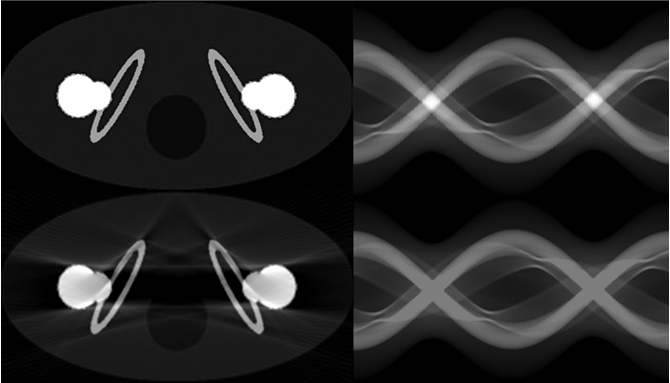
\includegraphics[scale=0.7]{img/artefact_generation}
\caption{{Upper left: Original Phantom; Upper right: Sinogram of the original phantom; 
Bottom Left: Restored corrupted sinogram; Bottom Right: Corrupted sinogram derived from the upper bound of the original sinogram.}}\label{artefact_generation}
\end{figure}

\section{Evaluation Procedure}

The comparison is realized in quantitative and qualitative way. The qualitative part is based on the visual analyses of the image and its sinogram.

The quantitative is composed by five index that determine how much similar are two images and the analysis of the intensity of the pixel along a line in the figure.

The index used are: 
\begin{itemize}
\item MSE: Mean Squared Error
\[ MSE = E[(I_{cor}-I_{ref})^2] \]
Where $I$ represents the pixel intensity.

\item PSNR: Peak-Signal-to-Noise Ratio
\[PSNR = 10\log_{10}\left({\frac{max^2(I_{ref})}{MSE}}\right) \]
Bigger is this value, more similar are the images

\item NCC: Normalized Correlation Coefficient
\[NCC = E\left[\frac{(I_{cor}-\mu_{cor})(I_{ref}-\mu_{ref})}{\sigma_{cor}\sigma_{ref}}\right] \]
Where $\mu$ and $\sigma$ are the mean and standard derivation of the image.
Nearest one, more similar are them

\item MSSIM: Mean Structure Similarity Index
\[MSSIM = E[SSIM] \]
\[ SSIM = \frac{(2\mu_{ref}\mu_{cor}+c_1)(2\sigma_{ref}\sigma_{cor}+c_2)}{(\mu_{ref}^2 +\mu_{cor}^2+c_1)(\sigma_{ref}^2+\sigma_{cor}^2+c_2)} \]
Where  $\mu$ and $\sigma$ are the mean and standard derivation of a window, and  $c_1$ and $c_2$ are two constants.
This index show the similarity with respect to the human vision. Nearest one, better.

\item FSIM: Feature Similarity Index
\end{itemize}

These five index, are calculated in 2 different regions which can be seen in the figure \eqref{region}. While, the line used to compare the intensity can be seen in the figure \eqref{line};

\begin{figure}[h]
\centering
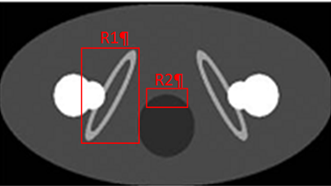
\includegraphics[scale=0.64]{img/region}
\caption{{Regions to calculate the index}}\label{region}
\end{figure}

\begin{figure}[h]
\centering
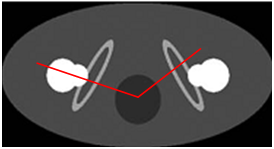
\includegraphics[scale=0.79]{img/line}
\caption{{Pixel Intensity Line}}\label{line}
\end{figure}

\section{Bertalmio at el.}
Initially we well do a analysis of the method of Bertalmio at el. and how it change with the tuning parameters K and the dilation of the inpainting domain:

\begin{figure}[h]
\centering
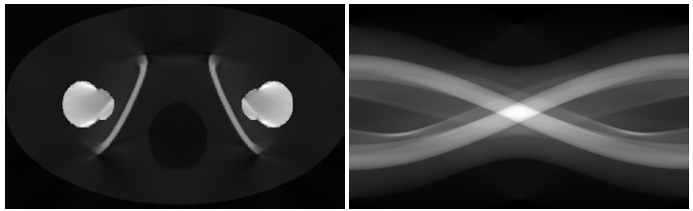
\includegraphics[scale=0.7]{img/bertalmio_basic}
\caption{{A tunned Bertalmio et al interpolation. Dilatation = 8 and k=10}}\label{bertalmio_basic}
\end{figure}

\begin{adjustwidth}{-1in}{-1in}
\centering
\begin{tabular}{c|c|c|c|c|c|c|c|c|c|c|}
\cline{2-11}
& \multicolumn{5}{|c|}{Region 1} & \multicolumn{5}{|c|}{Region 2} \\
\cline{2-11}
& MSE & PSNR & CC & MSSIM & fsim  & MSE & PSNR & CC & MSSIM & fsim  \\
\hline
\multicolumn{1}{|c|}{Artifact} & 4.262	& 17.567 &0.920	&0.338	&0.974	&1.121	&3.349	&0.159	&0.000	&0.936 \\
\multicolumn{1}{|c|}{Bertalmio} & 6.360	&15.828	&0.882	&0.400	&0.936	&0.024	&20.020	&0.959	&0.574	&0.981 \\
\hline
\end{tabular}
\end{adjustwidth}
\medskip

The method of Bertamio is capable to retrieve the information in the middle of the image, represented by the region two, but appear a new artifact on the region one. In the graph \eqref{line_bertalmio} is easy to see that the method of Bertalmio ignore the existence of the bone nearest of the metal. However, it 'fix' the problem that appeared between the two implants, in the artifact image we have negative values on this region, while on the Bertalmio image the intensity is almost equal to the reference. 

\begin{figure}[H]
\centering
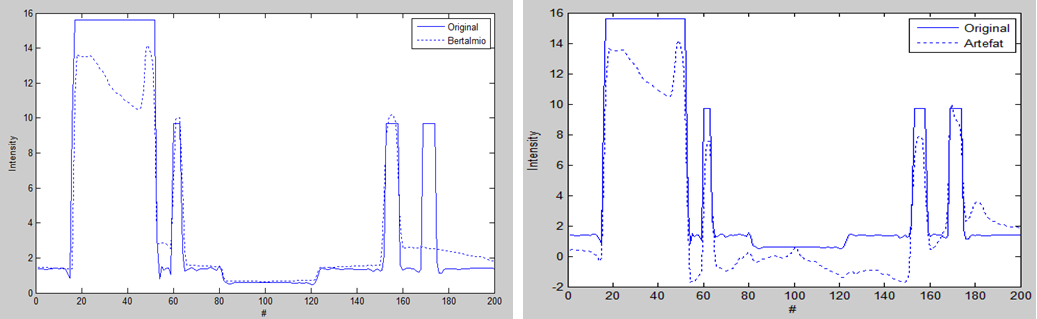
\includegraphics[scale=0.45]{img/line_bertalmio}
\caption{{Line comparison between restored(Bertalmio) image (left) and corrupted image(right).}}\label{line_bertalmio}
\end{figure}

\subsection{Parameter Dil}
The parameter Dilatation (Dil) is difficult to tuning, this happens because each image need a different one and it don't have a well defined tendency. The way that we use to chose this parameters is trial and error, obvious this method is very inefficient due to the high execution time of each try.

\begin{figure}[H]
\centering
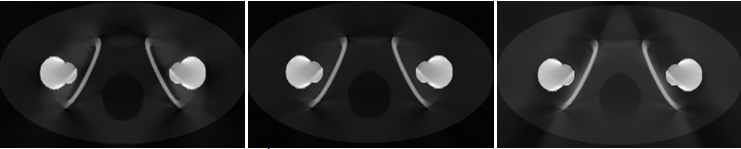
\includegraphics[scale=0.6]{img/dil_comp}
\caption{{Dil comparison. Dil=4(left) Dil=8(middle) Dil=12(right)}}\label{dil_comp}
\end{figure}

\begin{figure}[H]
\centering
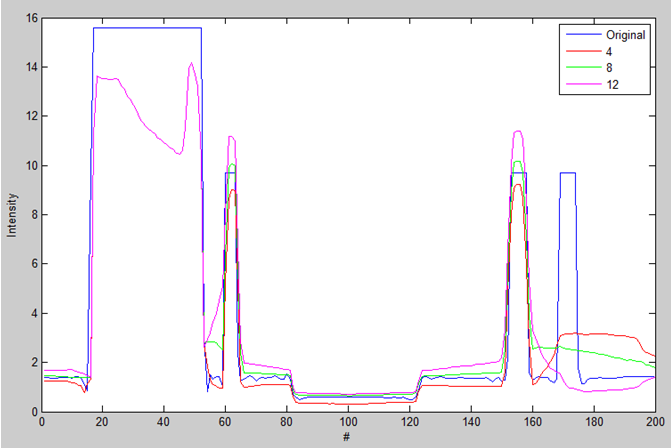
\includegraphics[scale=0.7]{img/dil_line}
\caption{{Dilatation line comparison}}\label{dil_line}
\end{figure}

The graph \eqref{dil_line} show the reason for the difficult to set the parameter, if the parameters is smaller or greater than a optimal is not possible judge if a better solution is reach increasing or decreasing it. The general rule is take the the shortest possible one ,in such way, the majority part of the artifact are surrounded.

\subsection{Parameter K}
The parameter of stabilization K has a important role of guarantee the convergence. Despite, in theory, a larger parameter K increase the error, it didn't happened in our case, since the blur edge filter make up the error. Furthermore, K interferes direct on the time of convergence of the method, as shown on the graph 

\begin{figure}[H]
\centering
\includegraphics[scale=0.66]{img/k_time}
\caption{{Convergence time x K}}\label{k_time}
\end{figure}

\subsection{Linear x Bertalmio}

\begin{figure}[H]
\centering
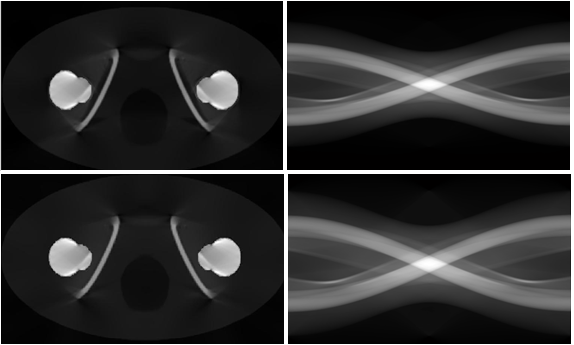
\includegraphics[scale=0.7]{img/linear_bertalmio}
\caption{{Upper side: Linear restoration. Botton side: Bertalmio et al restoration }}\label{linear_bertalmio}
\end{figure}

\begin{adjustwidth}{-1in}{-1in}
\centering
\begin{tabular}{c|c|c|c|c|c|c|c|c|c|c|}
\cline{2-11}
& \multicolumn{5}{|c|}{Region 1} & \multicolumn{5}{|c|}{Region 2} \\
\cline{2-11}
& MSE & PSNR & CC & MSSIM & fsim  & MSE & PSNR & CC & MSSIM & fsim  \\
\hline
\multicolumn{1}{|c|}{Artifact} & 4.262	& 17.567 &0.920	&0.338	&0.974	&1.121	&3.349	&0.159	&0.000	&0.936 \\
\multicolumn{1}{|c|}{Linear} &6.047	&16.047	&0.894	&0.381	&0.933	&0.065	&15.691	&0.979	&0.631	&0.981 \\
\multicolumn{1}{|c|}{Bertalmio} & 6.360	&15.828	&0.882	&0.400	&0.936	&0.024	&20.020	&0.959	&0.574	&0.981 \\
\hline
\end{tabular}
\end{adjustwidth}
\medskip

\begin{figure}[H]
\centering
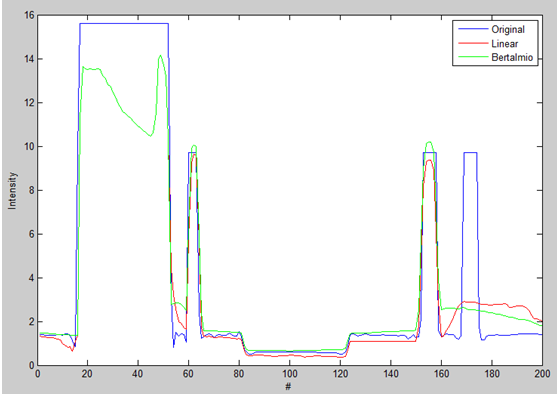
\includegraphics[scale=0.7]{img/line_linear_bertalmio}
\caption{{Line comparison between the Linear and Bertalmio et Al interpolation}}\label{line_linear_bertalmio}
\end{figure}

Comparing the two methods we can arrive a two conclusions: On the phantom hip, the two methods is almost equivalent, they have the same problem on the bone near to the metal implant and the remainder part is very similar to the original image. The linear method is slight better considering the the image edges ( see the pixel 60 and 160 on graph \eqref{line_linear_bertalmio}).

\section{Fusion}

The second analysis is regard to the fusion method. On this method there are two restoration process, so we will use all possible combination and compare then. The combination are Linear/Linear, Linear/Bertalmio, Bertalmio/Linear and Bertalmio, Bertalmio.
The fusion method has two parameters, n and t. We test how them change the restoration only for the case Linear/Linear, after we extrapolate the better parameters for the other cases.

\subsection{Parameter t}

The parameter t is the most important to set accordingly, because if it's low the fusion method don't work, and if is high the artifact is not removed.

\begin{figure}[H]
\centering
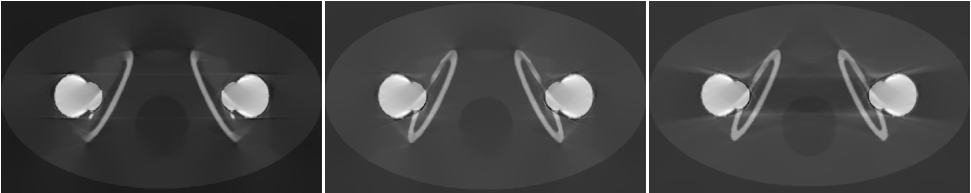
\includegraphics[scale=0.5]{img/t_image}
\caption{{t comparison. t=0.15(left) t=0.45(middle) t=0.75(right)}}\label{t_image}
\end{figure}

\subsection{Parameter n}

The parameter n is relevant, however is not fundamental set it to the right value. The prove show us that the best parameter depend of the region, additionally the difference are negligible , so we choose a intermediary parameter.

\begin{figure}[H]
\centering
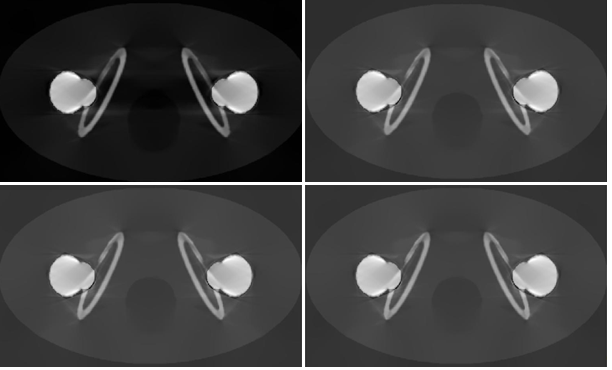
\includegraphics[scale=0.7]{img/n_image}
\caption{{n comparison. n=1(top/left) n=5(top/right) n=10(down/left) n=20(down/right)}}\label{n_image}
\end{figure}

\begin{adjustwidth}{-1in}{-1in}
\centering
\begin{tabular}{c|c|c|c|c|c|c|c|c|c|c|}
\cline{2-11}
& \multicolumn{5}{|c|}{Region 1} & \multicolumn{5}{|c|}{Region 2} \\
\cline{2-11}
& MSE & PSNR & CC & MSSIM & fsim  & MSE & PSNR & CC & MSSIM & fsim  \\
\hline
\multicolumn{1}{|c|}{Artifact} & 4.262	& 17.567 &0.920	&0.338	&0.974	&1.121	&3.349	&0.159	&0.000	&0.936 \\
\multicolumn{1}{|c|}{1} &4.382	&17.446	&0.930	&0.396	&0.965	&0.482	&7.017	&0.816	&0.135	&0.963 \\
\multicolumn{1}{|c|}{5} &4.426	&17.403	&0.924	&0.411	&0.964	&0.025	&19.879	&0.917	&0.418	&0.962 \\
\multicolumn{1}{|c|}{10} &4.307	&17.520	&0.926	&0.436	&0.965	&0.035	&18.456	&0.915	&0.418	&0.961 \\
\multicolumn{1}{|c|}{20} &4.380	&17.448	&0.924	&0.426	&0.964	&0.038	&18.103	&0.900	&0.388	&0.959 \\
\hline
\end{tabular}
\end{adjustwidth}
\medskip

\begin{figure}[H]
\centering	
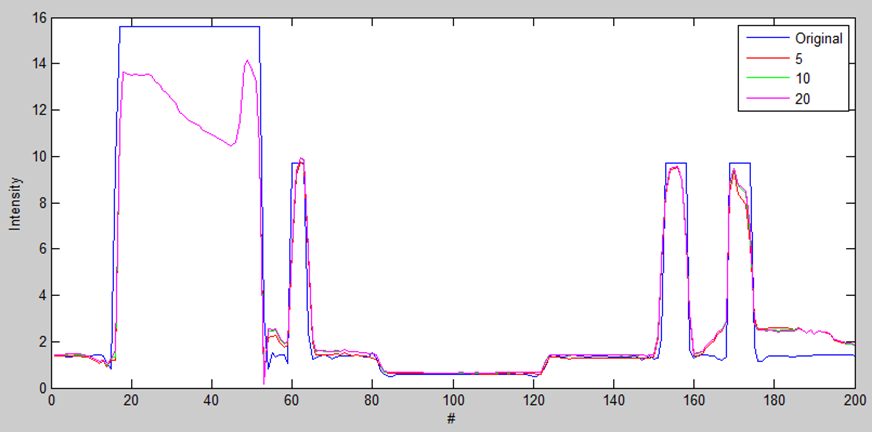
\includegraphics[scale=0.6]{img/n_line}
\caption{{Line comparison for diferent n parameters}}\label{n_line}
\end{figure}

\subsection{Combination Method}

\begin{figure}[H]
\centering
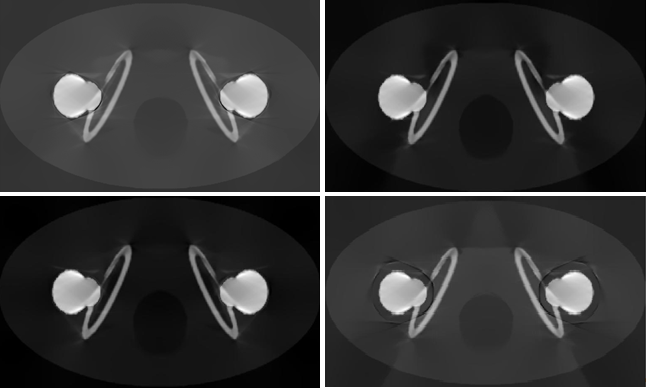
\includegraphics[scale=0.7]{img/method_comp}
\caption{{Method comparison. Linear/Linear(top/left) Bertalmio/Bertalmio(top/right) Linear/Bertalmio(down/left) Bertalmio/Linear(down/right)}}\label{method_comp}
\end{figure}

Qualitatively we can disregard the combination Bertalmio/Lin due to the clear additional artifact. The combination Bertalmio/ Bertalmio isn't acceptable as well, because of the high time consummation of the method.

\begin{adjustwidth}{-1in}{-1in}
\centering
\begin{tabular}{c|c|c|c|c|c|c|c|c|c|c|}
\cline{2-11}
& \multicolumn{5}{|c|}{Region 1} & \multicolumn{5}{|c|}{Region 2} \\
\cline{2-11}
& MSE & PSNR & CC & MSSIM & fsim  & MSE & PSNR & CC & MSSIM & fsim  \\
\hline
\multicolumn{1}{|c|}{Artifact} & 4.262	& 17.567 &0.920	&0.338	&0.974	&1.121	&3.349	&0.159	&0.000	&0.936 \\
\multicolumn{1}{|c|}{Lin/Lin} &4.380	&17.448	&0.924	&0.426	&0.964	&0.038	&18.103	&0.900	&0.388	&0.959 \\
\multicolumn{1}{|c|}{Ber/Ber} &3.866	&17.989	&0.935	&0.512	&0.970	&0.009	&24.236	&0.970	&0.643	&0.982 \\
\multicolumn{1}{|c|}{Lin/Ber} &3.768	&18.102	&0.943	&0.498	&0.969	&0.049	&16.925	&0.981	&0.681	&0.984 \\
\multicolumn{1}{|c|}{Ber/Lin} &4.315	&17.513	&0.918	&0.397	&0.962	&0.397	&7.861	&0.886	&0.272	&0.962 \\
\hline
\end{tabular}
\end{adjustwidth}
\medskip

\begin{figure}[H]
\centering	
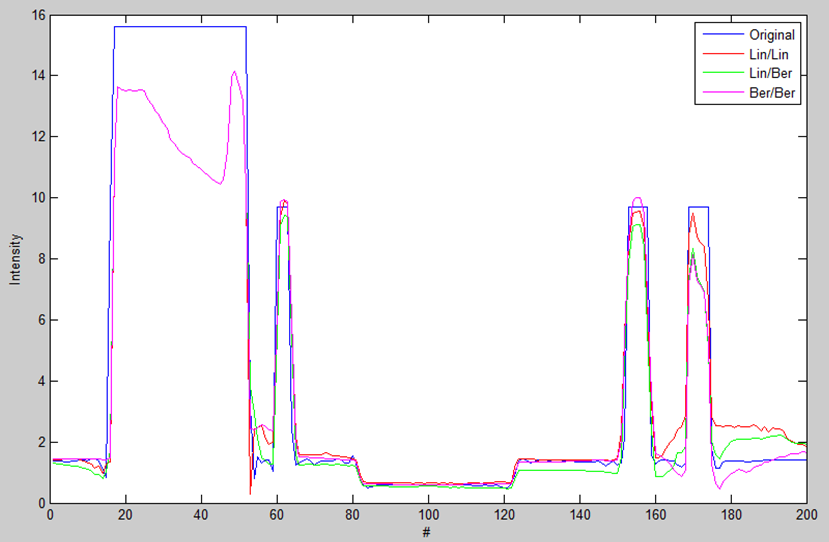
\includegraphics[scale=0.6]{img/line_method}
\caption{{Line comparison for different methods}}\label{line_method}
\end{figure}

The results show us that there isn't a method that surpass the other. Depending of the regions a method is better or not. For instance, the method Linear/Bertalmio have the lowest MSE, however between the pixel 120 and 150 the error is very high.

\section{Final analysis}

The phantom hip was a good image to test the method. Using it we arrived to two conclusions:

The method of Bertalmio is not a good method when the inpainting domain is large. It is not surprising because if we have less information, the estimate will be courser, thus don't have much sense use a method that require more time to execute a finer estimate.

Differently, the fusion method performed very well and the goal of retrieve the loss of information was achieved. However, some artifact arise. It can be a problem or not, all depend of which part the doctor want to see to do the diagnostic.